\documentclass[11pt,UKenglish, a4paper]{article}
\usepackage[utf8]{inputenc}
%--fonts--
\usepackage[T1]{fontenc}
\usepackage[bitstream-charter]{mathdesign}

%--packages--
\usepackage[UKenglish]{babel}
\usepackage{csquotes,textcomp,varioref}

%--Sitater i starten av dokumentet--
\usepackage{epigraph}

%--Notater i margen og geometri for størrelse--
\usepackage{geometry}
\usepackage{marginnote}

\usepackage{graphicx}
%--color--
\usepackage[dvipsnames]{xcolor}

%Setter inn pdfer
\usepackage[final]{pdfpages}

%-linespace--
\linespread{1.3}

%-Mer advansert liste--
\usepackage{enumitem}

%--hyperlinks-- include 
\usepackage[colorlinks=false, pdfborder={0 0 0}]{hyperref}

%--include subfiles-- 
\usepackage{subfiles}

%--fullpage--
%\usepackage{fullpage}

%--Uio-Front-Page--
%removed until it works \usepackage{ifikompendiumforside}

%--bibliography- -sortlocale=nb_No,
\usepackage[backend=biber, sortcites, defernumbers, style=numeric-comp, maxnames=2, natbib=true, backref, sorting=none, url=false]{biblatex}
%fjernet ifra style=authoryear-icomp
\addbibresource[datatype=bibtex]{Remote.bib}

%farger jeg skal ha med
\definecolor{myY}{RGB}{241, 196, 15}
\definecolor{myB}{RGB}{52, 152, 219}
\definecolor{myG}{RGB}{46, 204, 113}
\definecolor{myLy}{RGB}{149, 165, 166}
\definecolor{myR}{rgb}{231, 76, 60}

%--Author and Title--
\author{Simon Lysne Hyenes}

\title{Participatory Design}

%--Latex Optimalization--
\tolerance = 5000
\hbadness = \tolerance
\pretolerance = 2000
\begin{document}
\section{Participatory Design}

Participatory design is a research field and design methodology with a special focus on involving users as co-designers in design process. Participatory design has it's roots in the 1970 Scandinavian workplace democracy movement. Participatory design has evolved since the 1970's but it's core value still remains; those affected by a design should have a say in the design process\cite{Simonsen2012Routledge}.

Greenbaum frames PD within a political perspective where ``people have the right to influence their own lives''\cite[p.~39]{Hagen2010Social}. This democratic imperative refocuses the design process and emphasises ``genuine participation''\cite[p.~5]{Robertson2006Ethical}. 
\textit{Genuine participation} of future users and stakeholders expands the possible design space and radically changes the role of designers. 

Kristen Nygaard pionered the field by working with the Norwegian Iron and Metal Workers Union (NJMF). The goal was to increase both technical and organizational competence among the union workers. Workers feared that their needs where neglected by managements use and implementation of new technology. Early researchers aimed to balance power between management and workers \cite[p~.170]{Kensing1998Participatory}. These efforts has become the Scandinavian approach wih a ``Marxist commitment to democratically empowering workers and fostering democracy in the workplace''\cite[p.~164]{Spinuzzi2005Methodology}. Kensing and Greenbaum point to three theoretical roots: political economy, democracy and feminism\cite[p.~31]{Kensing2013Heritage}. 


Participatory design has since broadened it's scope and adapted to new issues beyond work/management relations and system development. Today it's used in many different contexts, such as architecture, policy and urban planning\cite[p.~2]{Velden2014RePoliticising}. 

Kensing and Greenbaum guiding principles reflect the heritage of PD while encompassing current practice:
\begin{itemize}
\item{Equalizing power relations}
\item{Democratic practices}
\item{Situation based actions}
\item{Mutual learning}
\item{Tools and techniques}
\item{Alternative visions about technology}
\end{itemize}\cite[p.~33-34]{Kensing2013Heritage}
These princicples are intertwined and facilitate each other. Bratteteig et. al. points to three core principles: ``Having a say, Mutual learning, Co-realisation''. Participation and democracy are enabled by users having a say through \textit{genuine participation}. Participation and having a say in itself is not enough, participants have to be given legitimate decision power and access to understand the problem area. To work on equal terms there has to be a shared language and socio-cultural understanding\cite[p.152]{Loewgren2004Thoughtful}.  

Designing the design process is by many considered just as important as the outcome. PD draws upon phenomenological view where every new design practice is unique. Each design practice requires different participants, skills and knowledge domains. The designers role is then as a skilled facilitator whom aims to involve the participants as co-designers.   
  
PD is especially appropriate at the earlier stages of the design. To fully utilize co-design with participants means involving users as early as possible.  Allowing users to participate during the ``fuzzy front-end''\cite[p.~6]{Sanders2008CoCreation} gives them access before constraints and visions steer the design process\cite{Loewgren2004Thoughtful}. 

\subsection{Tools and Techniques}
PD projects often lead to knowledge about tools and techniques that support these principles. Kensing and Blomberg point to that PD as a community of practice is shaped and defined by the tools and techniques employed: ``strategies that allow for the direct participation of workers in project definition and design specification.''\cite[p.~181]{Kensing1998Participatory}. Research in PD often strive to develop and formulate these strategies for future use. 

Tools and techniques can be judged by their ability to enable enacting, telling and making. Telling refers to participants ability to having a say. Making activities use creativity to explore future possibilities. Enacting refers to staging and imagining scenarios, allowing participants to enage with future situation and raise mutual understanding\cite[p.149]{Simonsen2012Routledge}. There are several prominent tool and techniques such as future workshop, probes, design games, and storyboards.
Low-fidelity prototyping is a central technique in PD and used in most projects. Contrary to other design practices prototyping of artifacts may not be specifically aimed at creating better prototypes but as boundary objects for discussion and envisioning futures.

PD also means taking the needs of the participants seriously. This mean that workshops and other engagements with users need to be engaging and fun. Formal, stiff and strictly procedural techniques are therefore less useful than techniques that engage through playing and doing.\cite[p.153]{Loewgren2004Thoughtful}. Experience and ability to facilitate such work requires both theoretical but also practical knowledge.The ability to converse, lead, guide and raise creativity and engagement essential and Löwgren and Stolterman stress the need to consider practical understanding as a valuable skill\cite[p.152]{Loewgren2004Thoughtful}. 

\subsection{Why PD in this project}
The main benefit of using PD is in the belief that the process will lead to not only a better solution but also a learning process of working with teenagers.

The scope and access means that the project participatory possibilities are limited. This project does not have the possibility to truly utilize participatory design. Despite this PD still offers valuable tools and techniques and an unique research focus. 


Bratteteig and Stolterman frame the purpose of design as:

``not just the designed artefact itself, but changes in the range of possibilities for action in the social organization which will use the artefact''\cite[p.~4]{Bratteteig1997Design}.

Beyond its morals implication this also points to PD ability to engage and work with specific design situations. Its specificity can positively focus and frame loosely defined design problems.  

The group we are working towards are teenage patients which have a unique situated perspective. The group can be considered domain experts with an understanding of their lifeworld, their wishes, concerns and needs. Cooperation with this group allows for an unique insight and a mutual learning process. The research area involved gaining insight into this domain beyond what I could envision or garner from literature. Technology, culture and society has changed in such ways that envisioning and imagination based techniques fail to capture or reflect these teenagers lifeworlds. 

Participatory design does not mean that the produced artifacts is the \textit{right} solution or reflect all future use situations. However involving future user raises the possibilities of ``that the product represent the values and meaning of the future users''\cite[p.3]{Velden2014Participatory}. Participatory design on alternative vision also enables escaping trends and the limitations of designers ``technical heritage''\cite{Feng2008Thinking}. 


\subsection{Design Cycle}
\begin{figure}[DesignProcess]
    \centering
	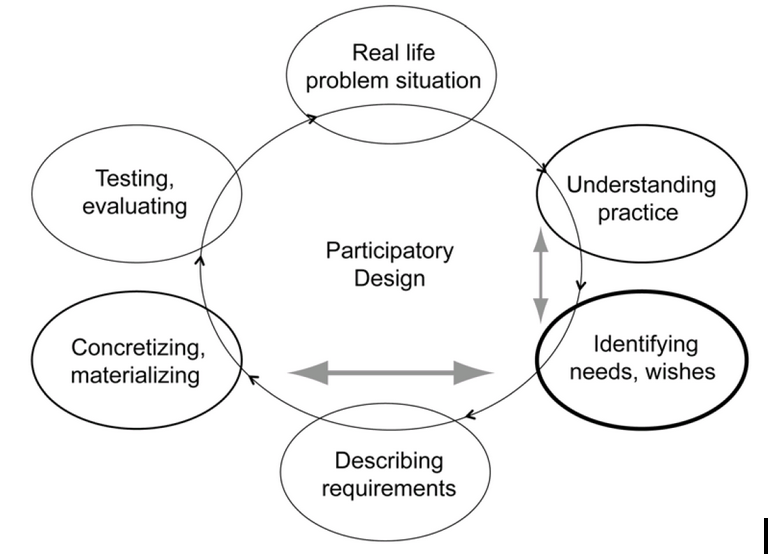
\includegraphics[width=0.5\linewidth]{DesignProcess}
    \caption{The use-oriented design cycle \cite[p~.128]{Bratteteig2013Organising}}
    \label{The use-oriented design cycle}
\end{figure}
There are several design approaches in PD, in this project I am using the use-oriented design cycle. Each stage in the cycle involves different considerations and tools and techniques. The cycle iterates and interplay between identifying needs and concretizing solutions. This reflect Schön's interplay between ``reflection-in-action'' and ``reflection-in-use''\cite[p.~23]{Loewgren2004Thoughtful}.

\subsection*{Ethics}

From a modern view PD values are related to the ethical stand ``that recognizes the accountability of design to the world it creates and the lives of those who inhabit them''\cite[p.~5]{Simonsen2012Routledge}. As mentioned every design practice is unique. The aim is to allow for \textit{genuine participation}. In doing so meant choosing amongst tools and techniques, focuses and crucially how to frame and present the project's goals. 

To truly benefit from using PD I tried to involve the users early in the design process. In the beginning this involved focusing the research on the participants lifeworlds and how they related to the proposed problem area. 
The tools and techniques chosen had to both engage the users but also facilitate mutual learning. This also involves not taking early design decision and instead facilitating the users ability to both explore future vision but also allow for co-realization\cite[p.~10]{Velden2014Participatory}. 

Considering Dewey’s ``morality in action''\cite[p.~70]{Robertson2006Ethical} every small decisions, soft-coercions, indifference, inclusion/exclusion has a moral and ethical consequence. These choices are ultimately the faciliatators responsibility. Bratteteig et. al discuss \textit{model power}, the symbolic power of the worldviews of the interpreter\cite[p.129]{Bratteteig2013Organising}. The designers role as facilitator and interpretator means that I had to consider my own model-monopoly over the situation. This involved reflecting upon how I related to and understood the user group and their needs. This reflection is especially important considering that the data is inscribed with my interpretations and values. 

Van der Velden and Mörtberg view PD as a value-centered design approach\cite[p.6]{Velden2014Participatory}. They point to that while PD doesn't ``frontload'' certain values it does enable emerging values through participation and through its methods. In this project certain values are front-loaded by the projects focus while others are implicitly or instrumental such as organizational rules. Van der Velden and Mörtberg describe the ``contact-zone'' as where the design process confronts different interpretations of values and moral. This pluralism means participants and faciliatators may differ in opinion and understanding of certain values\cite[p.~8]{Velden2014Participatory}.

\section{Outcomes}
In involving younger patient in the design process and using them as co-designers has several implications. Primarily is the loss of predictability in design solutions. Promoted ideas may contradict or seem foreign. Further divergent solution may come forth within the group. Settling for one coherent vision isn't always possible or practical.

The solutions will also reflect the lack of involvement of other stakeholders. Their inability to affect what is and isn't within the design space can be both a restriction and a freedom. In this project parents, health professionals and others were neglected to instead focus the limited resources on the patient group. 

\end{document}